% !TEX root =  ../supplementary.tex

\section{Parameter Estimates for the PRIAS dataset}
\label{sec : param_estimates_jm_fit_prias}
The posterior parameter estimates for the joint model we fitted to the PRIAS dataset are shown in \ref{tab : PSA_long} (longitudinal sub-model) and \ref{tab : PSA_survival} (relative risk sub-model), and parameter estimates for the variance-covariance matrix from the longitudinal sub-model are the following:
\begin{equation*}
\bmath{D} = \begin{bmatrix}
       0.409 & 0.105 & -0.140 \\[0.3em]
       0.105 & 1.725 & 0.431 \\[0.3em]
       -0.140 & 0.431 & 1.326
     \end{bmatrix}
\end{equation*} 
The effect of age only affects the baseline $\log_2 \mbox{PSA}$ score. However it is so small that it can be ignored for all practical purposes. Since the longitudinal evolution of $\log_2 \mbox{PSA}$ is modeled with non-linear terms, the interpretation of the coefficients corresponding to time is not straightforward. In lieu of the interpretation, in Web Figure \ref{fig : fitted_trend_psa} we present the fitted evolution of PSA over a period of 10 years for a hypothetical patient who was included in AS at the age of 70 years.

\begin{figure}[!htb]
\centerline{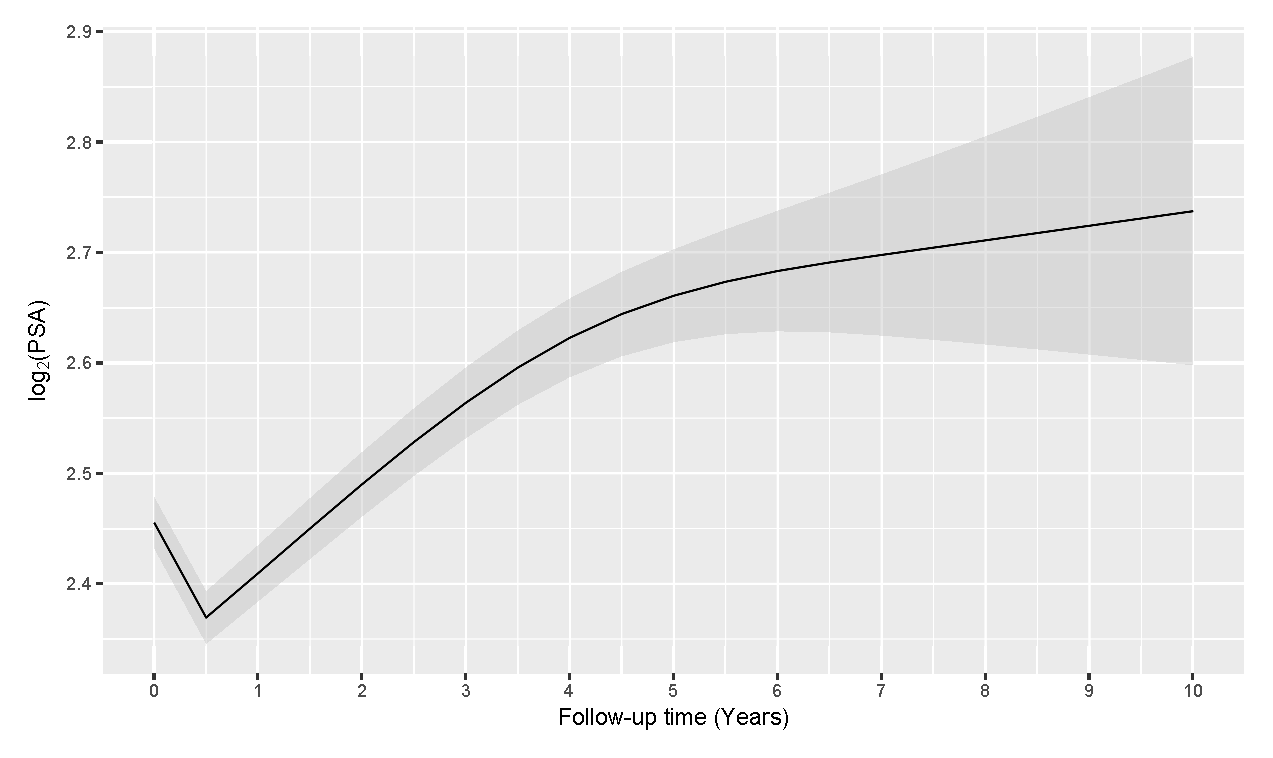
\includegraphics[width=\columnwidth]{images/fitted_trend_psa.eps}}
\caption{Fitted evolution of $\log_2 \mbox{PSA}$ over a period of 10 years with 95\% credible interval, for a hypothetical patient who was included in AS at the age of 70 years.}
\label{fig : fitted_trend_psa}
\end{figure}

\begin{table}[!htb]
\begin{center}
\caption{Longitudinal sub-model estimates for mean and 95\% credible interval, for the joint model fitted to the PRIAS dataset.}
\label{tab : PSA_long}
\begin{tabular}{lrrrrr}
\Hline
& Mean   & Std. Dev           & 2.5\%               & 97.5\%              & P              \\ \hline
Intercept                            &  2.455 & 0.012 & 2.433 & 2.480               & \textless0.000 \\
$(\mbox{Age} - 70)$                         & 0.003 & 0.001 & 4.9 $\times 10^{-4}$ & 0.006 & 0.032          \\
$(\mbox{Age} - 70)^2$       & -0.001 & 1.4 $\times 10^{-4}$ & -0.001 & -3.5 $\times 10^{-4}$ & \textless0.000 \\
Spline: visitTimeYears{[}0.0, 0.1{]}   & -0.006 & 0.012 & -0.031 & 0.017 & 0.674 \\
Spline: visitTimeYears{[}0.1, 0.5{]} & 0.228 & 0.019 & 0.192 & 0.265               & \textless0.000 \\
Spline: visitTimeYears{[}0.5, 4.0{]} & 0.140 & 0.029 & 0.088 & 0.197               & \textless0.000 \\
Spline: visitTimeYears{[}4.0, 7.0{]}   & 0.303 & 0.039 & 0.227 & 0.379               & \textless0.000 \\
$\sigma$                               & 0.324 & 0.001 & 0.321 & 0.326              &  \\ \hline
\end{tabular}
\end{center}
\end{table}

\clearpage

For the relative risk sub-model, the parameter estimates in \ref{tab : PSA_survival} show that only $\log_2 \mbox{PSA}$ velocity and the age at the time of inclusion in AS are strongly associated with the hazard of GR. For any patient, an increase in $\log_2 \mbox{PSA}$ velocity from -0.07 to 0.12 (first and third quartiles of the fitted velocities, respectively) corresponds to a 1.55 fold increase in the hazard of GR. A 10 year increase in the age at the time of inclusion in AS corresponds to a 1.44 fold increase in the hazard of GR. The effect of $\log_2 \mbox{PSA}$ value is small enough to be safely ignored for all practical purposes.

\begin{table}[!htb]
\begin{center}
\caption{Relative risk sub-model estimates for mean and 95\% credible interval, for the joint model fitted to the PRIAS dataset.}
\label{tab : PSA_survival}
\begin{tabular}{lrrrrr}
\Hline
Variable                      & Mean   & Std. Dev & 2.5\%  & 97.5\%                 & P              \\ \hline
$(\mbox{Age} - 70)$                    & 0.037 & 0.006 & 0.025 & 0.0490                  & \textless0.000 \\
$(\mbox{Age} - 70)^2$   & -0.001 & 0.001 & -0.003 & 1.8 $\times 10^{-4}$ & 0.104          \\
$\log_2 \mbox{PSA}$                  & -0.049 & 0.064 & -0.172 & 0.078 & 0.414         \\
Slope($\log_2 \mbox{PSA}$)           & 2.407 & 0.319 & 1.791 & 3.069 & \textless0.000 \\
\hline
\end{tabular}
\end{center}
\end{table}